%%%%%%%%%%%%%%%%%%%%%%%%%%%%%%%%%%%%%%%%%%%%%%%%%%%%%%%%%%%%%%%%%%%%%%%%%%%%%%%%%
%																				%
% ELEN4006 Project.tex														%
%																				%
%                       Ntsako Manyike (18 May 2011)							%
%																				%
%           Measurements Project								%
%                                                                               %
% Note: Minor modifications were made to the original paper                     %
%       by KJ Nixon 2005/10/12 (with permission from the original author        %
%																				%
%%%%%%%%%%%%%%%%%%%%%%%%%%%%%%%%%%%%%%%%%%%%%%%%%%%%%%%%%%%%%%%%%%%%%%%%%%%%%%%%%

\documentclass[10pt,twocolumn]{witseiepaper}

%
% All KJN's macros and goodies (some shameless borrowing from SPL)
\usepackage{KJN}
\usepackage{rotating}

%
% PDF Info
%
\ifpdf
\pdfinfo{
/Title (MEASUREMENTS PROJECT)
/Author (Ntsako Kennedy Manyike)
/CreationDate (D:201105180245)
/ModDate (D:201106040800)
/Subject (Final Report)
/Keywords ()
}
\fi

%%%%%%%%%%%%%%%%%%%%%%%%%%%%%%%%%%%%%%%%%%%%%%%%%%%%%%%%%%%%%%%%%%%%%%%%%%%%%%%
\begin{document}


\title{MEASUREMENTS PROJECT}

\author{Ntsako Manyike}

\thanks{School of Electrical \& Information Engineering, University of the
Witwatersrand, Private Bag 3, 2050, Johannesburg, South Africa}



%%%%%%%%%%%%%%%%%%%%%%%%%%%%%%%%%%%%%%%%%%%%%%%%%%%%%%%%%%%%%%%%%%%%%%%%%%%%%%%
%
\abstract{}

\keywords{Automated stage, LSM, microscope, X-Y linear motor}


\maketitle
\thispagestyle{empty}\pagestyle{empty}


%%%%%%%%%%%%%%%%%%%%%%%%%%%%%%%%%%%%%%%%%%%%%%%%%%%%%%%%%%%%%%%%%%%%%%%%%%%%%%%
%
\section{INTRODUCTION}

If you cannot measure it, you cannot control it. If you cannot control it, you cannot manage it. if you cannot manage it, you cannot improve it.
A transducer changes one form of energy to another. Sensors are the natural inputs to a measurement system, producing electrical signals that directly interface to the signal-conditioning element. Every measurement has a target-a physical parameter of interest. Termed the measurand, this is what drives the entire measurement process. The measurand could be a certain property of a material or a condition of a process.   In each case a single sensor or a collection of sensors is needed to selectively transduce the desired measurand. The electrical signals from the sensors are input to the instrumentation chain to ultimately produce the measurement of the measurand.
Piezoelectric measuring systems are active electrical systems. The application of mechanical stress to piezoelectric material will result in an electric field, and this effect is called Direct Piezoelectric Effect. Hence, when a force is applied on piezoelectric structure, this structure will generate an analog voltage signal between its electrodes. So, based on the value of generated voltage on piezoelectric sensor, the magnitude of applied force is measured.
Piezoelectric sensors are useful for measurement of force, pressure, acceleration and so on. The advantage of piezoelectric sensors compared with other types of sensors are their long life without aging, high sensitivity, low threshold, wide measuring range, practically displacement-free measurement, high natural frequency and a wide temperature range amongst other things.
%%%%%%%%%%%%%%%%%%%%%%%%%%%%%%%%%%%%%%%%%%%%%%%%%%%%%%%%%%%%%%%%%%%%%%%%%%%%%%%%
\section{BACKGROUND}

\subsection{Weight measurement systems}

The diagnosis of Tuberculosis and Malaria involves the examination of sputum
and blood samples respectively \cite{phppo,biotec,STimes}.  These examinations
also reveal the contagious quality of infections such as TB.  Therefore,
faster diagnosis results in better containment of the disease and allows the

%%%%%%%%%%%%%%%%%%%%%%%%%%%%%%%%%%%%%%%%%%%%%%%%%%%%%%%%%%%%%%%%%%%%%%%%%%%%%%%
\subsubsection*{Resistive:}

The six TTL logic level PWM signals formed inputs into a six channel class-D
amplifier.  This consisted of a primary stage in which comparators, made from
TL074 op-amps, pushed the voltage signals to the rails.  Thereafter, the same
TIP122 and TIP125 complimentary darlington transistor pairs were used in an
H-bridge configuration to provide current amplification.

It is typically understood that the armature windings filter Voltage Source
Inverter PWM signals to produce smoothed current signals.  In reality, the
-3 dB frequency of the filter created by the armature windings is given by
$f=\frac{R}{2\pi L}$.  For the designed armatures, the resultant -3 dB
frequencies were 3.183 kHz and 17.683 kHz for the wire-wound and PCB armatures
respectively.  Therefore, the switching frequency permeated through the
armatures as current signals with no attenuation.  A six channel filter bank
was designed to compensate for this effect.  Each channel was a second order
RLC filter, as shown in \figref{fig:Filter}.  The resulting -3 dB frequency was
112 Hz.

\begin{figure}[hb]
	\centering
		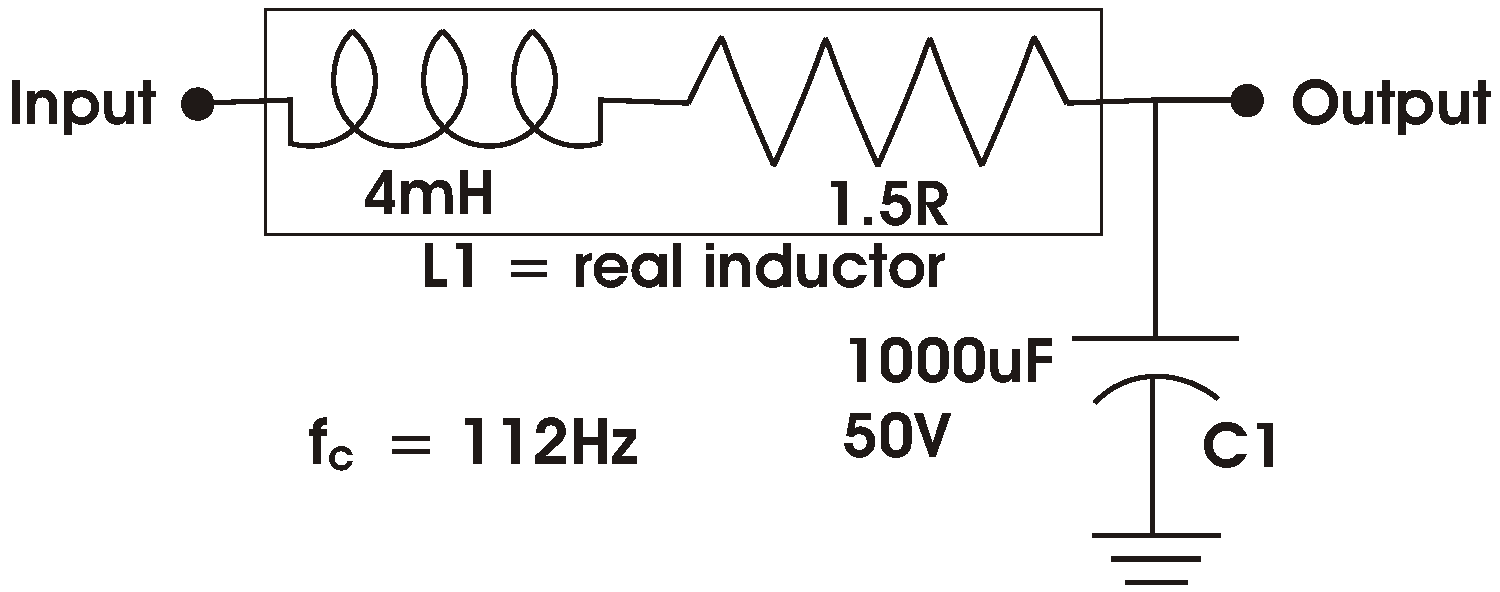
\includegraphics[width=0.45\textwidth]{../../Drawings/Filter.pdf}
	\caption{RLC Filter Circuit}
	\label{fig:Filter}
\end{figure}

%%%%%%%%%%%%%%%%%%%%%%%%%%%%%%%%%%%%%%%%%%%%%%%%%%%%%%%%%%%%%%%%%%%%%%%%%%%%%%%
\subsubsection*{Elastic:}

The topology employed consisted of an active armature and a passive PM
cursor \cite{Linsync}.  The advantage of this topology was that the cursor was
electrically isolated from the stage such that no electrical contacts were in
motion.  This increased durability.


where:

\begin{tabular}{lll}
& $v$      & = Linear Velocity (mm/s)\\
& $v_s$    & = Synchronous Linear Velocity (mm/s)\\
& $f$      & = Input Frequency (Hz)\\
& $\tau$   & = Pole Pitch (mm) \\
\end{tabular}

Two armatures were tested.  The first design made use of a PCB.  The second
was a wire-wound armature.  The advantages and disadvantages of both are
presented in \tabref{tab:Armatures} with a final specification given in
\tabref{tab:Specs}.  The two PM arrays shown in \figref{fig:PM} were also
tested.  They represent compromises between size and flux linkage.

%%%%%%%%%%%%%%%%%%%%%%%%%%%%%%%%%%%%%%%%%%%%%%%%%%%%%%%%%%%%%%%%%%%%%%%%%%%%%%%
\subsubsection*{Pneumatic:}

To determine the pole-pitch, the speeds required must be considered.  From the
Olympus BX50's technical data, the observable fields-of-view range between
0.22 mm and 5.5 mm.  From this, and the rate of capture of the digital imaging
devices, the linear speeds at which this system can move are between 0.176
mm/s and 44 mm/s.  This includes a 20\% overlap which allows for accurate
digital knitting.

%%%%%%%%%%%%%%%%%%%%%%%%%%%%%%%%%%%%%%%%%%%%%%%%%%%%%%%%%%%%%%%%%%%%%%%%%%%%%%%
\subsubsection*{Piezoelectric:}

To achieve these low speeds, minimisation of both the pole-pitch and the input
frequencies is essential.  The relationship between these three variables is
given in \eqnref{eqn:Speed}.  The pole-pitch was limited by the dimensions of
available Nd-Fe-B PM's.  The smallest available PM's were \mbox{8.6 $\times$
8.6 mm $\times$ 3 mm}, polarised along their shortest dimension. To minimise
force-ripple, the ratio of the magnet-length to the machine pole-pitch is
0.8 \cite{Tubular}.  This ratio results in reduced harmonics in the DC magnetic
field and lower thrust, but is essential for smooth motion. Therefore, the
system pole-pitch was 10.75 mm and the excitation frequencies needed to be
between 0.008 Hz and 2 Hz.
\begin{equation}
	v = v_s = 2f\tau
	\label{eqn:Speed}
\end{equation}

%%%%%%%%%%%%%%%%%%%%%%%%%%%%%%%%%%%%%%%%%%%%%%%%%%%%%%%%%%%%%%%%%%%%%%%%%%%%%%%
\section{System overview}

A microscope stage is required to move along all three axes.  The vertical
motion of the stage provides a focusing mechanism and is usually performed by
moving the stage mounting system vertically.  The specimen is then moved in
the X-Y plane, about the optical centre of the microscope stage, exposing any
point of the specimen to the viewer.  On the Olympus BX50, this motion is
provided by two concentric rotary dials.
 

%%%%%%%%%%%%%%%%%%%%%%%%%%%%%%%%%%%%%%%%%%%%%%%%%%%%%%%%%%%%%%%%%%%%%%%%%%%%%%%
\section{MODELLING}

The Olympus BX-50 has adopted standard photomicrography camera lenses, namely
C- and CS-mounted lenses \cite{Olympus}.  The capture rate of available
digital capture devices range between 1/60 fps, from still cameras, to 30 fps,
from video cameras using the National Television Standards Committee (NTSC)
system \cite{Olympus}.

%%%%%%%%%%%%%%%%%%%%%%%%%%%%%%%%%%%%%%%%%%%%%%%%%%%%%%%%%%%%%%%%%%%%%%%%%%%%%%%
\subsection{Sensing Element}

LSM's have come into favour because of \cite{Halbach-1,XY-Thrust}:
\begin{enumerate}
	\item Their accurate positioning capabilities via DC excitation.
	\item The lower cost and weight of permanent magnet (PM) movers which do not require power supplies
	\item The high thrusts, speeds and efficiencies they can provide.
	\item The absence of a transmission which eliminates gearing losses, and increases reliability and dynamic performance.
\end{enumerate}

%%%%%%%%%%%%%%%%%%%%%%%%%%%%%%%%%%%%%%%%%%%%%%%%%%%%%%%%%%%%%%%%%%%%%%%%%%%%%%%
\subsection{Signal Conditioning}

\begin{figure}[ht]
	\centering
		
\includegraphics[width=0.45\textwidth]{../../Drawings/Flow-Diagram.pdf}
	\caption{System Overview}
	\label{fig:Sys}
\end{figure}
\figref{fig:Sys} depicts the three sections of the designed system.

The dsPIC30F6014 MCU \cite{Microchip} was used to control the motor.  In the
case of sinusoidal power signals, it presented digital signals to two
digital-to-analog converters (DAC).  For the application of PWM power signals,
six output-compare channels were used.

%%%%%%%%%%%%%%%%%%%%%%%%%%%%%%%%%%%%%%%%%%%%%%%%%%%%%%%%%%%%%%%%%%%%%%%%%%%%%%%
\subsection{Signal Processing}

Two 12-bit DAC's produced the A and C phases for both directions.  A sequence
of inverting summing amplifiers generated the third phase from the redundancy
in three-phase systems, and provided bipolar operation.  Six Class-AB power
amplifiers provided the current necessary to drive the X-Y LSM.

%%%%%%%%%%%%%%%%%%%%%%%%%%%%%%%%%%%%%%%%%%%%%%%%%%%%%%%%%%%%%%%%%%%%%%%%%%%%%%%
\subsection{Data Communication}

A six channel class-D amplifier provided the current necessary to drive the
X-Y LSM through a filter bank. The filter bank was developed to compensate for
the armature's low filtering ability.

The armature windings were based on two flat, stacked, orthogonal LSM's as
described by Davies \cite{Simon}, providing independent two-dimensional
movement.

%%%%%%%%%%%%%%%%%%%%%%%%%%%%%%%%%%%%%%%%%%%%%%%%%%%%%%%%%%%%%%%%%%%%%%%%%%%%%%%
\section{SYSTEM ANALYSIS}

The LSM was a single sided design, employed to minimise the height of the
system.  The disadvantage of this design was that less flux was
generated \cite{Linsync}.  A back iron was also neglected because of the
associated weight which could not be accommodated by the stage support.  This
reduced flux linkage.

%%%%%%%%%%%%%%%%%%%%%%%%%%%%%%%%%%%%%%%%%%%%%%%%%%%%%%%%%%%%%%%%%%%%%%%%%%%%%%%
\subsection{Static Properties}

\begin{figure}[hb!]
	\centering
		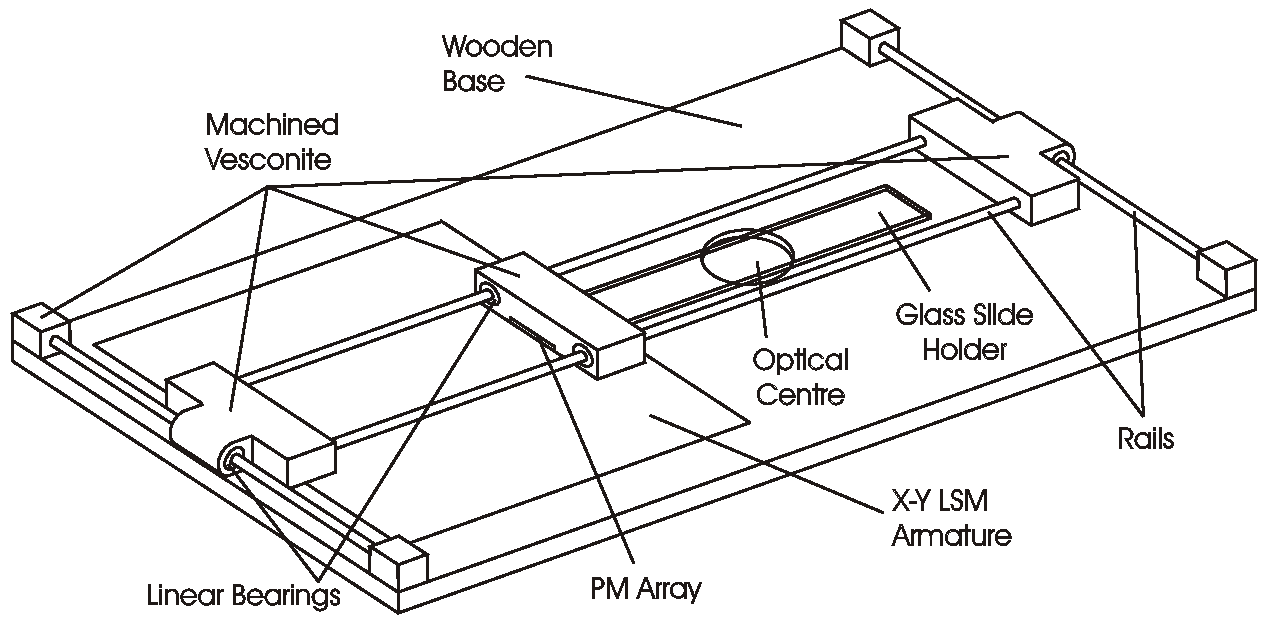
\includegraphics[width=0.50\textwidth]{../../Drawings/Stage-Final.pdf}
	\caption{Stage Design}
	\label{fig:Stage}
\end{figure}

%%%%%%%%%%%%%%%%%%%%%%%%%%%%%%%%%%%%%%%%%%%%%%%%%%%%%%%%%%%%%%%%%%%%%%%%%%%%%%%
\subsubsection*{Resolution:}

The layout specified by Davies \cite{Simon} was scaled for use in this
application.  The LSM's orthogonal placement provided independent motion along
two dimensions because of the associated orthogonal magnetic fields and
theoretical zero mutual inductance.  The disadvantage of this layout was that
the individual LSM's were at different depths from the cursor.  The result was
that, at the level of the PM array, the lower LSM produced a weaker magnetic
field than the upper LSM.

%%%%%%%%%%%%%%%%%%%%%%%%%%%%%%%%%%%%%%%%%%%%%%%%%%%%%%%%%%%%%%%%%%%%%%%%%%%%%%%
\subsubsection*{Range:}

The armature was a slotless design.  Although the magnetic field was weaker in
this design, the detent forces were eliminated \cite{Tubular,XY-Thrust}.
Detent forces are the periodic attractive forces between the PM's and the
metallic slots between the windings.  In order to achieve smooth motion, these
forces must be eliminated. 

%%%%%%%%%%%%%%%%%%%%%%%%%%%%%%%%%%%%%%%%%%%%%%%%%%%%%%%%%%%%%%%%%%%%%%%%%%%%%%%
\subsubsection*{System Error:}

%Placed Here so as to appear correctly
\begin{table*}[ht!]
	\centering
	\caption{Armature Advantages and Disadvantages}
		\begin{tabular}{lll}
			\hline
													&	{\msbf Advantages} 						& {\msbf Disadvantages}\\
			\hline
			{\msbf PCB}					& 1) The thin armature reduced leakage  			& 1) 24 series-turns/phase; costly to increase\\
													& flux and eliminated LSM vertical separation.& 2) High Cost (R3 000)\\
													& 2) The pole-pitch was exactly matched.\\													
			\hline
			{\msbf Wire-Wound}	& 1) Low Cost (R200)										& 1) Thicker armature increased leakage\\ 
													& 2) 180 series-turns/phase			& flux and imposed vertical LSM separation.\\
													& 3) Well matched pole-pitch  	& 2) Timely construction procedure.\\						\hline
		\end{tabular}
	\label{tab:Armatures}
\end{table*}


 

%Placed Here so as to appear correctly
\begin{table}[hb!]
	\centering
	\caption{Motor Specifications}
		\begin{tabular}{lll}
			\hline
           	 & {\msbf Specification} 	& {\msbf Value (Units)}\\
      \hline
          1. & 3$\Phi$ Connection   & $\Delta$\\
          2. & Pole Pairs							 & 6$\times$6\\
          3. & Pole Pitch							 & 10.75$\times$10.75 (mm)\\
          4. & PCB Track Width				 & 0.695 (mm)\\
          5. & PCB Series-Turns/Phase  & 24$\times$24\\
          6. & Wire-Wound wire $\oslash$   & 0.35 (mm)\\
          7. & Wire-Wound 						 & 180$\times$180\\
             & Series-Turns/Phase\\
          8. & Max Current   					 & 1.5 (A)\\
      		9. & Nd-Fe-B PM Size				 & 8.6$\times$8.6$\times$3 (mm)\\
      \hline
		\end{tabular}
	\label{tab:Specs}
\end{table}
\begin{figure}[htb!]
	\centering
		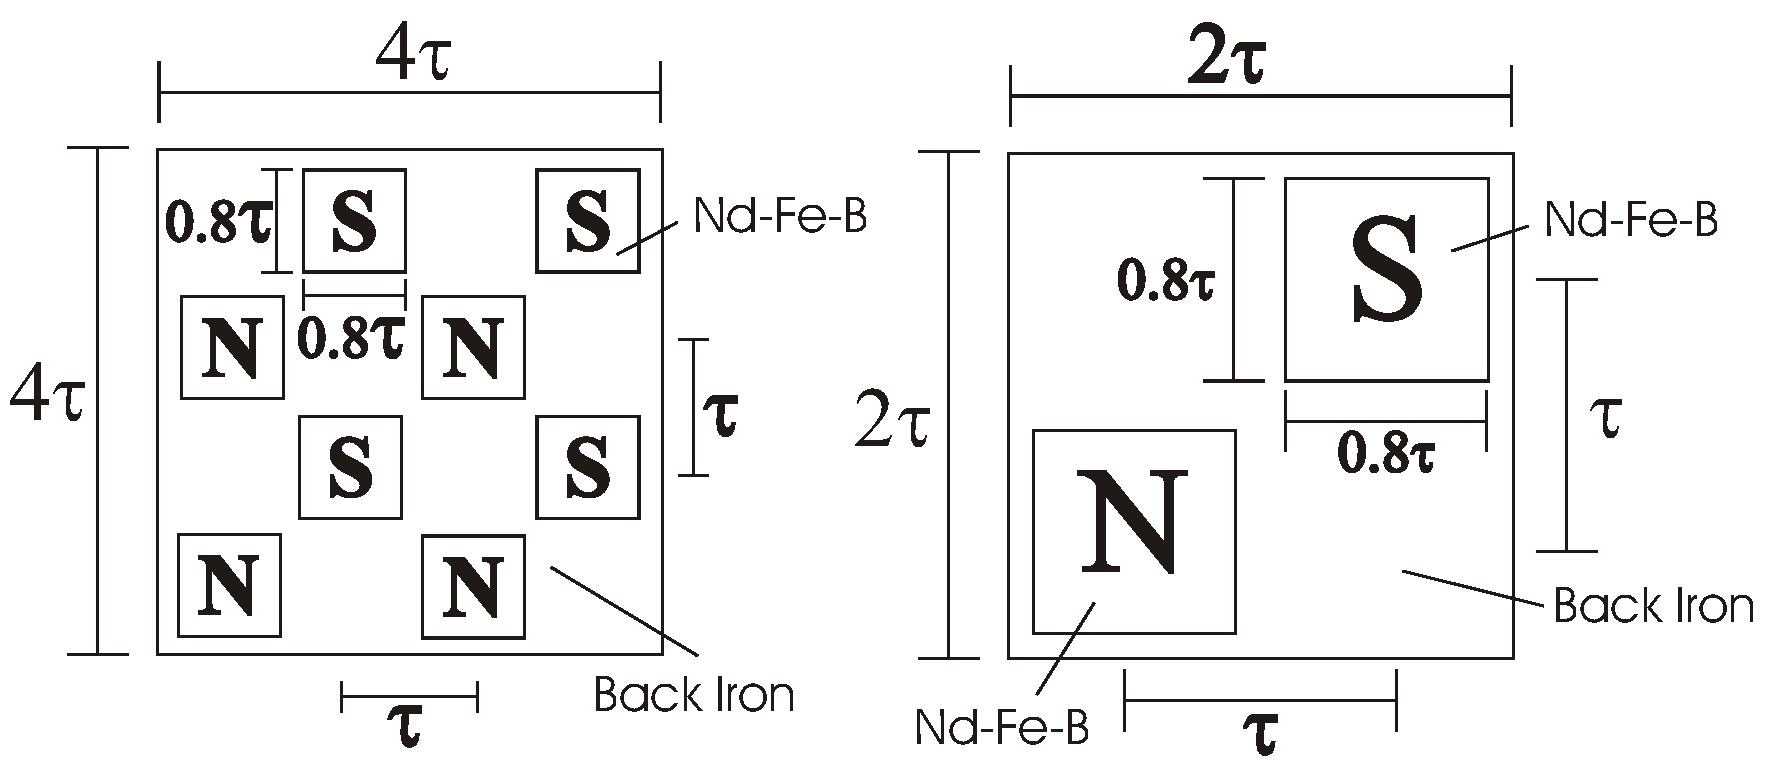
\includegraphics[width=0.48\textwidth]{../../Drawings/PM-Both.pdf}
	\caption{PM Array Configurations}
	\label{fig:PM}
\end{figure}
%%%%%%%%%%%%%%%%%%%%%%%%%%%%%%%%%%%%%%%%%%%%%%%%%%%%%%%%%%%%%%%%%%%%%%%%%%%%%%%
\subsection{Dynamic properties}

The dsPIC MCU was used to generate the six phase signals required to drive
both dimensions of the X-Y LSM.  The program strategy was designed according
to a layered system.  The signal generation formed the lowest level of the
structure and accepted two inputs, the X- and Y-direction frequencies, called
the frequency bus.  Subsequent layers existed separately from the generation
layer.  To control the LSM, a layer asserted a value onto the frequency bus.
This provided a means of stacking various layers such as a joystick or RS-232
controller layer.  

The two 12-bit digital buses were connected to two Maxim MX7847BN DAC's.
Channel A of the two DAC's produced phases A and C for the X-direction whilst
Channel B produced the same for the Y-Direction.  Bipolar operation was
achieved using inverting, summing, operational amplifier configurations
according to the application notes.  For each direction, phases A and C were
summed in an inverting configuration to produce phase B according to
\eqnref{eqn:3Phase}.  Tuning potentiometers were set to within 0.2\% fullscale
(FS) to achieve phase and amplitude symmetry.  The six phase signals formed
inputs to the six current gain amplifiers.  These were class-AB power
amplifier configurations using TIP122 and TIP125 complimentary darlington
transistor pairs.  They could be driven directly from the TL074 op-amps
because of their high current gain ($H_{fe-min}=1000$).  This eliminated
excessive external circuitry.  A TL074 op-amp was used to ensure accurate
amplification by placing the class-AB amplifier in the feedback loop of the
op-amp, with a buffered input to the op-amp.  The six outputs were connected
directly to the X-Y LSM windings.  \begin{eqnarray}
	i_A+i_B+i_C = 0\nonumber\\
	i_B = -i_A-i_C\label{eqn:3Phase}
\end{eqnarray}


%%%%%%%%%%%%%%%%%%%%%%%%%%%%%%%%%%%%%%%%%%%%%%%%%%%%%%%%%%%%%%%%%%%%%%%%%%%%%%%%%
\section{CONCLUSION}

Slow and smooth motion necessary for the automation of specimen
photomicrography could not be achieved due to torsional effects introduced
when only two X-Y linear synchronous motors were used to automate an electric
microscope stage. To resolve this problem, it is recommended that a layout
using four independent linear synchronous motors be implemented.
%%%%%%%%%%%%%%%%%%%%%%%%%%%%%%%%%%%%%%%%%%%%%%%%%%%%%%%%%%%%%%%%%%%%%%%%%%%%%%%%%
%\nocite{*}

\bibliographystyle{witseie}
\bibliography{references}

%%%%%%%%%%%%%%%%%%%%%%%%%%%%%%%%%%%%%%%%%%%%%%%%%%%%%%%%%%%%%%%%%%%%%%%%%%%%%%%


%{\tiny \vfill \hfill \today \hspace{5mm} witseie-paper-2003.\TeX}

\end{document}

" vim: ts=4
" vim: tw=78
" vim: autoindent
" vim: shiftwidth=4

